\documentclass[11pt]{article}
\usepackage{geometry,marginnote} % Pour passer au format A4
\geometry{hmargin=1cm, vmargin=1.5cm} % 

% Page et encodage
\usepackage[T1]{fontenc} % Use 8-bit encoding that has 256 glyphs
\usepackage[english,french]{babel} % Français et anglais
\usepackage[utf8]{inputenc} 

\usepackage{lmodern}
\usepackage[np]{numprint}
\setlength\parindent{0pt}

% Graphiques
\usepackage{graphicx,float,grffile}
\usepackage{tikz,pst-eucl,pst-plot,pstricks,pst-node,pstricks-add,pst-fun,pgfplots} 

% Maths et divers
\usepackage{amsmath,amsfonts,amssymb,amsthm,verbatim,scratch3}
\usepackage{multicol,enumitem,url,eurosym,gensymb,tabularx}

\DeclareUnicodeCharacter{20AC}{\euro}



% Sections
\usepackage{sectsty} % Allows customizing section commands
\allsectionsfont{\centering \normalfont\scshape}

% Tête et pied de page
\usepackage{fancyhdr} \pagestyle{fancy} \fancyhead{} \fancyfoot{}

%\fancyfoot[L]{Collège Faubert}
%\fancyfoot[C]{\thepage / 6}
%\fancyfoot[R]{Série Générale}

\renewcommand{\headrulewidth}{0pt} % Remove header underlines
%\renewcommand{\footrulewidth}{0pt} % Remove footer underlines

\newcommand{\horrule}[1]{\rule{\linewidth}{#1}} % Create horizontal rule command with 1 argument of height

\newcommand{\Pointilles}[1][3]{%
  \multido{}{#1}{\makebox[\linewidth]{\dotfill}\\[\parskip]
}}

\newtheorem{Definition}{Définition}

\usepackage{siunitx}
\sisetup{
    detect-all,
    output-decimal-marker={,},
    group-minimum-digits = 3,
    group-separator={~},
    number-unit-separator={~},
    inter-unit-product={~}
}

\setlength{\columnseprule}{1pt}


\begin{document}

\begin{center}
  \textit{Un tableau ne vit que par celui qui le regarde.} - \textbf{Pablo Picasso}
\end{center}

\begin{multicols}{2}\noindent
\subsubsection*{Ex1 - Calculer la moyenne}

$$12 \; ; \; 13 \; ; \; 16 \; ; \; 8 \; ; \; 9$$

\subsubsection*{Ex2 - Calculer la moyenne}

$$200 \; ; \; -40 \; ; \; 600 \; ; \; -36 \; ; \; 1\,200 \; ; \; -150$$
\end{multicols}


\begin{multicols}{2}\noindent
\subsubsection*{Ex3 - Calculer la moyenne pondérée}

\begin{itemize}[label={$\bullet$}]
  \item 13 coefficient 4. 
  \item 12 coefficient 1. 
  \item 6 coefficient 4. 
  \item 16 coefficient 3. 
\end{itemize} 

\subsubsection*{Ex4 - Calculer la moyenne d'âge des élèves}

\begin{itemize}[label={$\bullet$}]
  \item 42 élèves ont 10 ans.
  \item 72 élèves ont 11 ans.
  \item 120 élèves ont 12 ans.
  \item 116 élèves ont 13 ans.
  \item 82 élèves ont 14 ans.
\end{itemize} 
\end{multicols}


\subsubsection*{Pb1 - Une histoire de moyenne}

\begin{enumerate}
  \item[1.] Voici les notes de Cid : $15 \; ; \; 17 \; ; \; 9 \; ; \; 12 \; ; \; 7$.\\
  Calculer sa moyenne.
  \item[2.] Il repasse sa dernière évaluation et remplace le 7 par 12. \\
  Combien de points en plus va-t-il avoir sur sa moyenne ?
  \item[3.] Ses notes sont : $15 \; ; \; 17 \; ; \; 9 \; ; \; 12 \; ; \; 12$.\\
  Quelle note doit-il obtenir lors de la prochaine évaluation s'il souhaite obtenir 14 de moyenne ?
\end{enumerate}


\subsubsection*{Pb2 - Une histoire de moyenne pondérée}

\begin{multicols}{2}\noindent
Vincent a obtenu ces notes : 

\begin{itemize}[label={$\bullet$}]
  \item 11 coefficient 4. 
  \item 5 coefficient 2. 
  \item 7 coefficient 4. 
  \item 14 coefficient 2. 
\end{itemize} \columnbreak

\begin{enumerate}
  \item[1.] Calculer sa moyenne.
  \item[2.] Son professeur lui propose d'enlever une note parmi les quatre. \\
  Quelle la note est la plus intéressante à enlever afin d'obtenir la meilleure moyenne ?
\end{enumerate} 
\end{multicols}


\subsubsection*{Pb3 - Une histoire de tableur}

\begin{figure}[H]
  \centering
  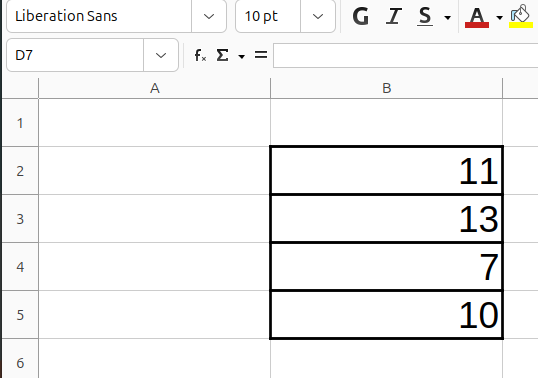
\includegraphics[width=0.5\linewidth]{5x4-statistiques/tableur.png}
\end{figure}

\begin{enumerate}
  \item[1.] Quelle formule taper pour calculer automatiquement la moyenne dans le tableur ?
\end{enumerate} 

\end{document}